% =====================================================================
\chapter{Optimización bayesiana}
\label{tema:4}
% =====================================================================

La optimización bayesiana usa el sustituto probabilístico del \cref{tema:3} para decidir el siguiente experimento: elige el punto que maximiza una \emph{función de adquisición}, una medida del valor esperado de ensayarlo según el modelo. El método procede de Jones, Schonlau y Welch~\cite{jones}, que introdujeron el algoritmo EGO con la mejora esperada; la exposición sigue la §4 del tutorial de Frazier~\cite{frazier}, los capítulos~7, 8 y~11 de Garnett~\cite{garnett}, la revisión de Shahriari \emph{et al.}~\cite{shahriari} y el capítulo~16 de Kochenderfer y Wheeler~\cite{kw}. Todo el tema trata problemas de \emph{minimización}; para maximizar basta cambiar el signo de $f$.

\section{El algoritmo}

\begin{algoritmo}[Optimización bayesiana]\label{alg:bo}
Datos: dominio $\X$, presupuesto $N$, diseño inicial de $n_0$ puntos.
\begin{enumerate}[label=\arabic*.]
  \item Evaluar el diseño inicial (por ejemplo, un LHS con $n_0\approx 10\,d$ o menos si el presupuesto es corto) y formar $\D_{n_0}$.
  \item Para $n=n_0,\dots,N-1$:
  \begin{enumerate}[label=(\alph*)]
    \item ajustar el sustituto a $\D_n$ (hiperparámetros por verosimilitud marginal);
    \item calcular $x_{n+1}\in\arg\max_{x\in\X}\alpha_n(x)$ con un optimizador auxiliar (varios arranques de L-BFGS-B o una nube de candidatos);
    \item evaluar $y_{n+1}=f(x_{n+1})+\varepsilon$ y añadir el par a los datos.
  \end{enumerate}
  \item Recomendar $\hat x_N\in\arg\min_{x}\mu_N(x)$ (entre los puntos evaluados o en todo $\X$) y confirmar con ensayos repetidos.
\end{enumerate}
\end{algoritmo}

La función de adquisición debe equilibrar dos tendencias: \emph{explotar} (ensayar donde la media $\mu_n$ es baja) y \emph{explorar} (ensayar donde la incertidumbre $\sigma_n$ es grande). En lo que sigue, $\mu=\mu_n(x)$, $\sigma=\sigma_n(x)$ es la desviación típica de la función latente $f(x)$ (no de una nueva observación) y $\fmejor$ es el valor de referencia: el mínimo observado si no hay ruido o el mínimo de $\mu_n$ en los puntos evaluados si lo hay~\cite[§5]{frazier}.

\section{Probabilidad de mejora}

\begin{definicion}[Probabilidad de mejora]\label{def:pi}
$\PI_n(x)=\Pr\bigl[f(x)<\fmejor-\xi\bigr]=\Phi\Bigl(\dfrac{\fmejor-\xi-\mu}{\sigma}\Bigr)$, con un margen $\xi\ge 0$.
\end{definicion}

La igualdad se debe a que $f(x)\sim\N(\mu,\sigma^2)$ y a la tipificación (módulo~0.8, §6.3). La PI ignora \emph{cuánto} se mejora: prefiere una mejora casi segura y diminuta a una probable y grande, y con $\xi=0$ tiende a muestrear junto al mejor punto actual~\cite[§7.5]{garnett}.

\section{Mejora esperada}

\begin{definicion}[Mejora y mejora esperada]\label{def:ei}
La \emph{mejora} en $x$ es $I(x)=\max\bigl(\fmejor-f(x),0\bigr)$, y la \emph{mejora esperada} es $\EI_n(x)=\E_n[I(x)]$, donde la esperanza se toma respecto a la posterior de $f(x)$ dados los datos~\cite[ec.~(14)]{jones}.
\end{definicion}

\begin{teorema}[Forma cerrada de la mejora esperada]\label{teo:ei}
Si $f(x)\mid\D_n\sim\N(\mu,\sigma^2)$ con $\sigma>0$ y $z=(\fmejor-\mu)/\sigma$, entonces
\[
\EI_n(x)=(\fmejor-\mu)\,\Phi(z)+\sigma\,\varphi(z).
\]
Si $\sigma=0$, $\EI_n(x)=\max(\fmejor-\mu,0)$.
\end{teorema}

\begin{proof}
Se escribe $f(x)=\mu+\sigma Z$ con $Z\sim\N(0,1)$. La mejora es positiva si y solo si $\mu+\sigma Z<\fmejor$, es decir, $Z<z$. Por tanto
\[
\EI_n(x)=\int_{-\infty}^{z}(\fmejor-\mu-\sigma t)\,\varphi(t)\,dt=(\fmejor-\mu)\int_{-\infty}^{z}\varphi(t)\,dt-\sigma\int_{-\infty}^{z}t\,\varphi(t)\,dt .
\]
La primera integral es $\Phi(z)$. Para la segunda, como $\varphi(t)=e^{-t^2/2}/\sqrt{2\pi}$ cumple $\varphi'(t)=-t\varphi(t)$, se tiene $\int_{-\infty}^{z}t\varphi(t)\,dt=\bigl[-\varphi(t)\bigr]_{-\infty}^{z}=-\varphi(z)$, porque $\varphi(t)\to0$ cuando $t\to-\infty$ (integral impropia convergente, módulo~0.6, §4.1). Sustituyendo, $\EI_n(x)=(\fmejor-\mu)\Phi(z)+\sigma\varphi(z)$. Si $\sigma=0$, $f(x)=\mu$ es constante y $I(x)=\max(\fmejor-\mu,0)$.
\end{proof}

Frazier~\cite[ec.~(8)]{frazier} da una forma equivalente para maximización, escrita con $\Delta=\mu-\fmejor$ y $[\Delta]^+$; Jones \emph{et al.}~\cite[ec.~(15)]{jones} la dan en la forma del teorema.

\begin{proposicion}[Propiedades de la mejora esperada]\label{prop:ei}
Como función de $(\mu,\sigma)$, con $\sigma>0$:
\begin{enumerate}
  \item $\EI>0$ y $\EI\ge\max(\fmejor-\mu,0)$;
  \item $\partial\EI/\partial\mu=-\Phi(z)<0$: a igual incertidumbre, se prefiere la media más baja;
  \item $\partial\EI/\partial\sigma=\varphi(z)>0$: a igual media, se prefiere la mayor incertidumbre.
\end{enumerate}
\end{proposicion}

\begin{proof}
(i) $I(x)\ge 0$ y es positiva con probabilidad $\Phi(z)>0$, luego su esperanza es positiva; por la desigualdad de Jensen (módulo~6, §2.1) aplicada a la función convexa $t\mapsto\max(\fmejor-t,0)$, $\E[I]\ge\max(\fmejor-\E f(x),0)$. (ii) y (iii): sea $g(\mu,\sigma)=\sigma\,h(z)$ con $h(z)=z\Phi(z)+\varphi(z)$, de modo que $\EI=g$. Como $h'(z)=\Phi(z)+z\varphi(z)+\varphi'(z)=\Phi(z)$, y $\partial z/\partial\mu=-1/\sigma$, $\partial z/\partial\sigma=-z/\sigma$, resulta $\partial g/\partial\mu=\sigma\Phi(z)(-1/\sigma)=-\Phi(z)$ y $\partial g/\partial\sigma=h(z)+\sigma\Phi(z)(-z/\sigma)=\varphi(z)$.
\end{proof}

\begin{ejemplo}[Tres candidatos para la inyectora]\label{ej:ei}
Tras varios ensayos, el mejor coste de referencia es $\fmejor=0{,}80$~€ y el modelo da, en tres candidatos, $A$: $\mu=0{,}78$, $\sigma=0{,}01$; $B$: $\mu=0{,}83$, $\sigma=0{,}06$; $C$: $\mu=0{,}95$, $\sigma=0{,}10$. Para $B$, $z=(0{,}80-0{,}83)/0{,}06=-0{,}5$, $\Phi(-0{,}5)=0{,}3085$ y $\varphi(-0{,}5)=0{,}3521$, luego
\[
\EI(B)=-0{,}03\cdot0{,}3085+0{,}06\cdot0{,}3521=-0{,}00926+0{,}02112=0{,}01187\ \text{€}.
\]
\begin{center}\small
\begin{tabular}{@{}lccccc@{}}
\toprule
Candidato & $z$ & $\PI$ & $\EI$ (€) & $\LCB=\mu-2\sigma$ (€) \\
\midrule
$A$ & $2{,}0$ & $0{,}9772$ & $0{,}02008$ & $0{,}76$ \\
$B$ & $-0{,}5$ & $0{,}3085$ & $0{,}01187$ & $0{,}71$ \\
$C$ & $-1{,}5$ & $0{,}0668$ & $0{,}00293$ & $0{,}75$ \\
\bottomrule
\end{tabular}
\end{center}
La PI y la EI eligen $A$, una mejora casi segura de unos dos céntimos; la cota inferior de confianza elige $B$, cuya media es peor pero que podría resultar mucho mejor. El candidato $C$, con más incertidumbre pero una media muy alta, no interesa a ninguna. La elección entre criterios es una elección sobre la actitud ante el riesgo.
\end{ejemplo}

\begin{figure}[ht]
\centering
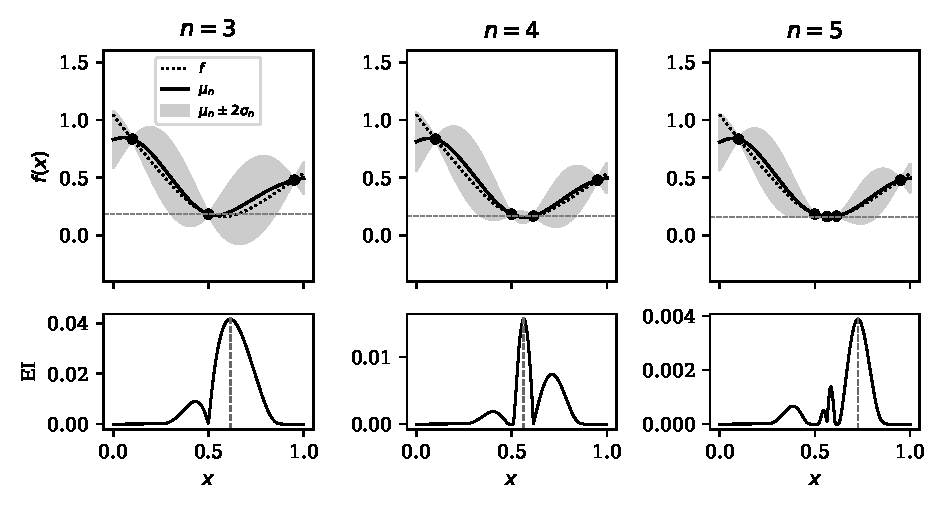
\includegraphics[width=\textwidth]{M25-fig-bo.pdf}
\caption{Tres iteraciones de optimización bayesiana con mejora esperada sobre una función de una variable (Parte~4 de la práctica). Arriba, la función verdadera (punteada), la media posterior y la banda $\pm2\sigma_n$; la línea discontinua horizontal es $\fmejor$. Abajo, la EI y el punto que maximiza (línea vertical). La EI se anula en los puntos ya evaluados y es grande donde la media es baja o la incertidumbre alta.}
\label{fig:bo1d}
\end{figure}

\section{Cotas de confianza y muestreo de Thompson}

\begin{definicion}[Cota inferior de confianza]\label{def:lcb}
Para un parámetro $\beta_n>0$, se elige $x_{n+1}\in\arg\min_x\LCB_n(x)$, con $\LCB_n(x)=\mu_n(x)-\sqrt{\beta_n}\,\sigma_n(x)$. En maximización se usa la cota superior $\UCB_n=\mu_n+\sqrt{\beta_n}\sigma_n$ (GP-UCB).
\end{definicion}

Srinivas \emph{et al.}~\cite{srinivas} demostraron que, con una sucesión $\beta_n$ que crece logarítmicamente, el regret acumulado de GP-UCB crece como $O^*\bigl(\sqrt{N\beta_N\gamma_N}\bigr)$, donde $\gamma_N$ es la máxima información que $N$ observaciones ruidosas pueden aportar sobre $f$; para el núcleo exponencial cuadrático, $\gamma_N$ crece como una potencia de $\log N$, y el regret medio $R_N/N$ tiende a cero. La teoría da una justificación al equilibrio entre explorar y explotar, pero los valores de $\beta_n$ que exige son conservadores; en la práctica se usan constantes entre $1$ y $9$~\cite[§8.4 y cap.~10]{garnett}.

El \emph{muestreo de Thompson} extrae una función $\tilde f\sim\GP(\mu_n,k_n)$ de la posterior y ensaya su mínimo; explora en proporción a la probabilidad de que cada punto sea el óptimo y se paraleliza con facilidad~\cite[§7.9]{garnett}.

\section{Optimizar la función de adquisición}

La función $\alpha_n$ es barata pero multimodal: vale casi cero en la mayor parte del dominio y tiene picos estrechos. Lo habitual es evaluarla en una nube de miles de candidatos (aleatorios y perturbaciones de los mejores puntos) y refinar los mejores con L-BFGS-B, usando su gradiente analítico o por diferenciación automática~\cite[§9.2]{garnett}, \cite{botorch}. Con valores de EI muy pequeños conviene trabajar con su logaritmo para evitar regiones numéricamente planas.

\begin{observacion}[Varianza latente y varianza predictiva]\label{obs:latente}
Muchas bibliotecas devuelven la desviación típica de una nueva \emph{observación}, $\sqrt{\sigma_n^2(x)+\sigma_\varepsilon^2}$, en lugar de la de $f(x)$. Usarla en la EI o en la probabilidad de cumplir una restricción es un error: en un punto ya ensayado la incertidumbre nunca baja del nivel de ruido, la EI no se anula y el algoritmo repite indefinidamente el mismo ajuste. En la práctica, con \texttt{GaussianProcessRegressor} y un \texttt{WhiteKernel}, hay que restar la varianza del ruido. En los experimentos de la práctica con la inyectora, sin esta corrección el algoritmo dedicaba la segunda mitad del presupuesto a repetir ajustes casi idénticos en una esquina del dominio.
\end{observacion}

\section{Restricciones}

\begin{proposicion}[Mejora esperada con restricciones]\label{prop:eic}
Sea el problema de la \cref{def:restricciones} con una restricción $c(x)\le 0$ modelada con un proceso gaussiano independiente del de $f$, con posterior $\N(\mu_c,\sigma_c^2)$, y sea $\fmejor$ el mejor valor \emph{factible}. La mejora restringida $I_c(x)=I(x)\,\mathbf 1[c(x)\le 0]$ tiene esperanza
\[
\EI_c(x)=\EI_n(x)\cdot\Phi\Bigl(\frac{-\mu_c(x)}{\sigma_c(x)}\Bigr).
\]
\end{proposicion}

\begin{proof}
Por la independencia de los dos procesos,\[\E\bigl[I(x)\,\mathbf 1[c(x)\le0]\bigr]=\E[I(x)]\,\Pr[c(x)\le 0],\]y $\Pr[c(x)\le0]=\Phi(-\mu_c/\sigma_c)$ por tipificación.
\end{proof}

Gardner \emph{et al.}~\cite{gardner} y Gelbart, Snoek y Adams~\cite{gelbart} estudian la optimización bayesiana con restricciones desconocidas colocando también un proceso gaussiano sobre cada restricción; el segundo admite además restricciones que se evalúan por separado del objetivo. El producto de la \cref{prop:eic} es la forma más sencilla de combinar ambos modelos~\cite[§11.2]{garnett}. Para una especificación $w(x)\le w_{\max}$, la probabilidad de cumplirla es $\Phi\bigl((w_{\max}-\mu_w)/\sigma_w\bigr)$. Si todavía no hay ningún punto factible, se maximiza solo la probabilidad de factibilidad~\cite[§11.2]{garnett}. Las restricciones conocidas y baratas no se modelan: se imponen al generar los candidatos.

\section{Evaluaciones por lotes}

En una planta se suelen hacer varios ensayos por turno, o hay varias máquinas: se necesita proponer $q$ puntos a la vez. La generalización natural es la \emph{mejora esperada multipunto}~\cite{ginsbourger},
\[
q\text{-}\EI(x^{(1)},\dots,x^{(q)})=\E_n\Bigl[\max\bigl(\fmejor-\min_{j}f(x^{(j)}),0\bigr)\Bigr],
\]
que no tiene forma cerrada útil y se estima por Monte Carlo con la distribución conjunta de los $q$ valores; BoTorch la optimiza con gradientes de Monte Carlo~\cite{botorch}. Dos heurísticas secuenciales más sencillas, de Ginsbourger, Le Riche y Carraro~\cite{ginsbourger}, eligen los puntos uno a uno añadiendo un dato ficticio en cada punto elegido: el \emph{creyente del kriging} usa como valor la media posterior $\mu_n(x^{(j)})$, y el \emph{mentiroso constante} usa un valor fijo $L$ (el mínimo, la media o el máximo observado; cuanto mayor es $L$, más se dispersan los puntos). Como la varianza posterior no depende de los valores (\cref{obs:posterior}), el dato ficticio reduce la incertidumbre alrededor de $x^{(j)}$ y aleja de él al siguiente punto del lote. Si los ensayos terminan en momentos distintos, los pendientes se tratan igual (optimización asíncrona~\cite[§11.4]{garnett}).

\section{Varios objetivos}

En la inyectora se puede querer, en lugar de un único coste, minimizar a la vez la fracción defectuosa y el tiempo de ciclo, y dejar la elección final a la dirección de la planta.

\begin{definicion}[Dominancia y frente de Pareto]\label{def:pareto}
Sean $F(x)=(F_1(x),\dots,F_m(x))$ objetivos a minimizar. El punto $x$ \emph{domina} a $x'$ si $F_i(x)\le F_i(x')$ para todo $i$ y $F_i(x)<F_i(x')$ para algún $i$. Un punto es \emph{óptimo de Pareto} si ningún otro lo domina; la imagen del conjunto de óptimos es el \emph{frente de Pareto}~\cite[§12.1]{kw}, \cite[§9.2]{mn}.
\end{definicion}

\begin{definicion}[Hipervolumen]\label{def:hv}
Dado un punto de referencia $r$ dominado por todos los puntos de interés, el \emph{hipervolumen} de un conjunto $P$ de vectores objetivo es la medida (área en dos dimensiones) de la región $\{v: \exists p\in P,\ p\le v\le r\}$ dominada por $P$ y acotada por $r$.
\end{definicion}

El hipervolumen crece si y solo si se añade un punto no dominado por el conjunto, y por eso es la medida habitual de progreso. La \emph{mejora esperada del hipervolumen} (EHVI) es la generalización de la EI; Daulton, Balandat y Bakshy~\cite{qehvi} la extienden a lotes con restricciones (qEHVI) y la calculan con diferenciación automática. Una alternativa más sencilla es escalarizar.

\begin{proposicion}[Escalarización de Chebyshev]\label{prop:chebyshev}
Sean $w_i>0$ pesos y $z^\star$ un punto ideal con $z^\star_i\le F_i(x)$ para todo $x$. Todo minimizador de $s_w(x)=\max_i w_i\bigl(F_i(x)-z^\star_i\bigr)$ es débilmente óptimo de Pareto: no existe $x'$ con $F_i(x')<F_i(x)$ para todo $i$.
\end{proposicion}

\begin{proof}
Si existiera tal $x'$, entonces $w_i(F_i(x')-z_i^\star)<w_i(F_i(x)-z^\star_i)$ para cada $i$, porque $w_i>0$; tomando el máximo en $i$ en ambos lados (el máximo de cantidades estrictamente menores es estrictamente menor), $s_w(x')<s_w(x)$, contra la minimalidad de $x$.
\end{proof}

ParEGO~\cite{parego} aplica la EI a la escalarización de Chebyshev aumentada con pesos aleatorios distintos en cada iteración, y así recorre el frente. A diferencia de la suma ponderada, la escalarización de Chebyshev alcanza también los puntos de las partes no convexas del frente (\cref{eje:4-chebyshev}).

\section{Varias fidelidades}

A menudo hay versiones más baratas e imprecisas del experimento: una simulación del llenado del molde antes del ensayo en máquina, un ensayo de resistencia a 7 días en lugar de 28, un entrenamiento corto en lugar de uno completo. La optimización multifidelidad modela conjuntamente $f(x,s)$, con $s$ la fidelidad, y elige a la vez el punto y la fidelidad~\cite[§11.5]{garnett}, \cite[§5]{frazier}. La regla más simple es dividir la adquisición por el coste: Snoek, Larochelle y Adams~\cite{snoek} proponen la mejora esperada por segundo, $\EI(x)/c(x)$, con el coste $c(x)$ también modelado. Kandasamy \emph{et al.}~\cite{kandasamy} (MF-GP-UCB) usan las fidelidades baratas para descartar regiones poco prometedoras y reservan las caras para las regiones buenas, con garantías de regret mejores que las de ignorar las aproximaciones.

\section{Caso de estudio: el optimizador de la inyectora}

\begin{ejemplo}[Optimización bayesiana con restricción de alabeo]\label{ej:bo-inyectora}
Se aplica el \cref{alg:bo} al \cref{ej:inyectora} (Parte~4 de la práctica; datos sintéticos). Diseño inicial: LHS de 10 lotes. Sustitutos: dos procesos gaussianos Matérn 5/2 con ARD y ruido estimado, uno para el coste observado y otro para el alabeo medido, ambos con entradas en $[0,1]^3$. Adquisición: EI restringida (\cref{prop:eic}) con la varianza latente (\cref{obs:latente}) y $\fmejor$ igual al mínimo de la media posterior entre los ensayos con probabilidad de cumplir el alabeo de al menos $0{,}5$. Optimización de la adquisición: 4000 candidatos uniformes y 500 perturbaciones gaussianas ($\sigma=0{,}05$) de puntos ya ensayados. Presupuesto: 20 lotes más. Recomendación: el mínimo de la media posterior del coste en $20\,000$ puntos del dominio entre los que tienen $\Pr[w\le0{,}45]\ge0{,}8$. Como referencia se toma la alternativa sin bucle: los 30 lotes en un único LHS y la misma recomendación. Con 10 repeticiones de cada estudio:
\begin{center}\small
\begin{tabular}{@{}lccccc@{}}
\toprule
 & regret & regret & alabeo rec. & lotes fuera & coste medio \\
Método (30 lotes) & mediano (€) & máximo (€) & máximo (mm) & de esp. & lotes (€) \\
\midrule
Optimización bayesiana & $0{,}0066$ & $0{,}0219$ & $0{,}448$ & $39\,\%$ & $0{,}828$ \\
LHS de 30 + PG & $0{,}0170$ & $0{,}0322$ & $0{,}451$ & $68\,\%$ & $0{,}841$ \\
\bottomrule
\end{tabular}
\end{center}
La optimización bayesiana reduce el regret mediano a menos de la mitad, todas sus recomendaciones cumplen la restricción (la del LHS en el peor caso la viola por $0{,}001$~mm), y además produce menos lotes fuera de especificación y más baratos durante el estudio: si los ensayos se hacen en producción, también gana en regret acumulado. Con lotes de dos ensayos por turno ($q=2$, creyente del kriging) el regret mediano es $0{,}0044$~€ en solo 10 rondas: en este problema, paralelizar no cuesta precisión. El regret de $0{,}0066$~€ por pieza supone, frente al óptimo, unos 6600~€ al año por millón de piezas, y el ahorro frente a la receta del operario es de más de $0{,}08$~€ por pieza.
\end{ejemplo}

\begin{table}[ht]
\centering\small
\begin{tabularx}{\textwidth}{@{}>{\raggedright\arraybackslash}p{2.5cm}>{\raggedright\arraybackslash}X>{\raggedright\arraybackslash}p{1.4cm}>{\raggedright\arraybackslash}p{3.8cm}@{}}
\toprule
Herramienta & Para qué sirve & Licencia & Cuándo elegirla \\
\midrule
BoTorch~\cite{botorch} & Adquisiciones de Monte Carlo: qEI, qNEI, qEHVI, multifidelidad, restricciones & MIT & Problemas a medida, lotes, varios objetivos \\
Ax~\cite{ax} & Interfaz de alto nivel sobre BoTorch: experimentos, restricciones de resultado, ensayos pendientes & MIT & Campañas reales con varias personas y máquinas \\
Optuna \texttt{GPSampler}~\cite{optuna} & Optimización bayesiana con PG dentro de Optuna & MIT & Si ya se usa Optuna \\
SMAC3~\cite{smac3} & BO con bosques aleatorios y espacios condicionales & BSD & Variables categóricas y jerárquicas \\
scikit-learn + SciPy & PG y optimización de la adquisición escritos a mano & BSD & Docencia y prototipos (práctica) \\
\bottomrule
\end{tabularx}
\caption{Tecnologías para la optimización bayesiana.}
\label{tab:tec4}
\end{table}

\begin{observacion}[Errores frecuentes en la práctica]\label{obs:errores4}
\begin{enumerate}
  \item Usar la varianza predictiva en lugar de la latente (\cref{obs:latente}).
  \item Tomar como $\fmejor$ el mínimo \emph{observado} con ruido: la maldición del ganador (\cref{prop:ganador}) hace la referencia demasiado optimista y la EI se vuelve tímida.
  \item Optimizar mal la adquisición (pocos candidatos, un único arranque): el algoritmo deja de explorar sin que nadie lo note.
  \item Diseño inicial demasiado pequeño: con 2 o 3 puntos los hiperparámetros son arbitrarios y las primeras decisiones, malas.
  \item Recomendar en la frontera de la restricción sin margen ni confirmación: la mitad de los lotes ensayados exactamente en el límite parecerán violarla (en la práctica, el $49\,\%$ en el óptimo).
  \item Confiar en la BO en dimensión alta (más de unas 20 variables) sin modelos específicos ni regiones de confianza.
\end{enumerate}
\end{observacion}

\begin{lecturas}
\item Jones, Schonlau y Welch~\cite{jones}, §4.1–4.2 (la mejora esperada y el algoritmo EGO).
\item Frazier~\cite{frazier}, §4.1 «Expected Improvement» y §5 «Exotic Bayesian Optimization».
\item Garnett~\cite{garnett}, §7.3, §7.5, §7.8–7.9, §8.2–8.4 y §11.2–11.7.
\item Kochenderfer y Wheeler~\cite{kw}, §16.3–16.6.
\item Shahriari \emph{et al.}~\cite{shahriari}, revisión general.
\end{lecturas}

\section*{Ejercicios del tema 4}
\addcontentsline{toc}{section}{Ejercicios del tema 4}

\begin{ejercicio}{1}{eje:4-pi}
(a) Explique por qué la PI con $\xi=0$ tiende a ensayar puntos pegados al mejor actual. (b) ¿Cuánto vale la EI en un punto ya evaluado si no hay ruido? ¿Y si lo hay y se usa por error la varianza predictiva? (c) ¿Qué representa $\beta_n$ en la LCB y qué ocurre en los límites $\beta_n\to0$ y $\beta_n\to\infty$?
\end{ejercicio}

\begin{ejercicio}{2}{eje:4-calculo}
Con $\fmejor=1{,}00$, calcule PI (con $\xi=0$), EI y $\LCB=\mu-2\sigma$ en los candidatos $P$: $\mu=0{,}98$, $\sigma=0{,}02$; $Q$: $\mu=1{,}05$, $\sigma=0{,}10$; $R$: $\mu=1{,}20$, $\sigma=0{,}30$. ¿Qué punto elige cada criterio? Use $\Phi(1)=0{,}8413$, $\varphi(1)=0{,}2420$, $\Phi(-0{,}5)=0{,}3085$, $\varphi(-0{,}5)=0{,}3521$, $\Phi(-2/3)=0{,}2525$, $\varphi(-2/3)=0{,}3194$.
\fuente{adaptado de Kochenderfer y Wheeler~\cite{kw}, §16.3–16.5 (texto del curso AA222/CS361 de Stanford~\cite{aa222}).}
\end{ejercicio}

\begin{ejercicio}{2}{eje:4-restringida}
En el candidato $A$ del \cref{ej:ei}, el modelo de alabeo da $\mu_w=0{,}44$~mm y $\sigma_w=0{,}02$~mm, con límite $0{,}45$~mm; en $B$, $\mu_w=0{,}40$ y $\sigma_w=0{,}02$. Calcule la EI restringida de ambos (use $\Phi(0{,}5)=0{,}6915$ y $\Phi(2{,}5)=0{,}9938$). ¿Cambia la elección?
\end{ejercicio}

\begin{ejercicio}{2}{eje:4-creyente}
Proceso gaussiano exponencial cuadrático con $\sigma_f=\ell=1$, sin ruido, con una observación en $x=0$. (a) Calcule $\sigma_1^2(0{,}5)$ y $\sigma_1^2(1)$. (b) El primer punto del lote es $x^{(1)}=1$; con el creyente del kriging se añade un dato ficticio en $x=1$. Calcule $\sigma^2(0{,}5)$ y $\sigma^2(1)$ después. (c) Explique por qué el resultado no depende del valor ficticio y por qué el segundo punto del lote ya no se elegirá en $x=1$.
\fuente{adaptado de Ginsbourger, Le Riche y Carraro~\cite{ginsbourger} y de Garnett~\cite{garnett}, §11.3 «Synchronous Batch Observations».}
\end{ejercicio}

\begin{ejercicio}{2}{eje:4-pareto}
Seis ajustes de la inyectora dan (defectos en \%, ciclo en s): $(2{,}0;30)$, $(3{,}0;26)$, $(5{,}0;22)$, $(4{,}0;27)$, $(8{,}0;21)$, $(2{,}5;32)$. (a) Determine el conjunto no dominado. (b) Calcule su hipervolumen respecto a $r=(10;35)$. (c) ¿Cuánto aumentaría el hipervolumen un nuevo punto $(4{,}0;23)$?
\fuente{adaptado de Kochenderfer y Wheeler~\cite{kw}, §12.1 «Pareto Optimality», y de Martins y Ning~\cite{mn}, §9.2.}
\end{ejercicio}

\begin{ejercicio}{2}{eje:4-coste}
Para decidir el siguiente ensayo de la inyectora se puede hacer una simulación de llenado (20~min de cálculo) cuya EI estimada sobre el coste real es $0{,}002$~€, o un lote en máquina (120~min) con EI $0{,}009$~€. (a) Compare la EI por minuto. (b) ¿Qué EI debería tener la simulación para que ambas opciones fueran equivalentes? (c) ¿Qué riesgo tiene este criterio si la simulación está sesgada?
\end{ejercicio}

\begin{ejercicio}{3}{eje:4-ei}
(a) Demuestre que $\EI(\mu,\sigma)\to\max(\fmejor-\mu,0)$ cuando $\sigma\to 0^+$. (b) Demuestre que $\EI$ es convexa en $\mu$ para $\sigma$ fijo. (c) Deduzca la fórmula de la EI cuando se maximiza: $I=\max(f(x)-\fmejor,0)$, y demuestre que puede escribirse como $[\Delta]^++\sigma\varphi(\Delta/\sigma)-\abs{\Delta}\,\Phi(-\abs{\Delta}/\sigma)$ con $\Delta=\mu-\fmejor$, forma usada por Frazier.
\fuente{adaptado de Frazier~\cite{frazier}, §4.1, y de Jones, Schonlau y Welch~\cite{jones}, §4.1.}
\end{ejercicio}

\begin{ejercicio}{3}{eje:4-chebyshev}
Un problema con dos objetivos tiene como conjunto alcanzable los puntos $F^{(1)}=(0;1)$, $F^{(2)}=(1;0)$ y $F^{(3)}=(0{,}6;0{,}6)$. (a) Compruebe que los tres son óptimos de Pareto. (b) Demuestre que ninguna suma ponderada $w_1F_1+w_2F_2$ con $w_i>0$ tiene a $F^{(3)}$ como minimizador. (c) Encuentre pesos de Chebyshev (con $z^\star=(0,0)$) para los que $F^{(3)}$ sea el único minimizador.
\end{ejercicio}
